\chapter{Fourier-Analyse}
Bei der Fourier-Analyse 
(\href{http://de.wikipedia.org/wiki/Joseph_Fourier}{Jean Baptiste Joseph Fourier}; 1768 - 1830) 
zerlegen wir eine 
periodische Funktion in Sinus-Schwingungen verschiedener Frequenzen.  Dieses Verfahren
wird in der Praxis zur Ton- und Bild-Verarbeitung eingesetzt.  Au{\ss}erdem ist die
Fourier-Analyse ein wichtiges Hilfsmittel zur L\"osung von Differential-Gleichungen.
Im Rahmen dieser Vorlesung werden wir die Fourier-Analyse allerdings nur zur Berechnung
unendlichen Reihen einsetzen, denn f\"ur die anderen Anwendungen reicht die Zeit 
nicht aus.

Bei der Fourier-Analyse gehen wir davon aus, dass eine Funktion 
$f:\mathbb{R} \rightarrow \mathbb{R}$ gegeben ist, die \emph{periodisch} mit der
Periode $2\cdot\pi$ ist, d.~h.~es gilt
\\[0.1cm]
\hspace*{1.3cm}
$\forall x \in\mathbb{R}: f(x+2\cdot\pi) = f(x)$.
\\[0.1cm]
Ein triviales Beispiel f\"ur eine periodische Funktion ist die konstante Funktion 
$x \mapsto c$.
Das typische Beispiel einer periodischen Funktion ist die Funktion
$x \mapsto \sin(x)$, denn es gilt $\sin(x+2\cdot\pi) = \sin(x)$.  Genauso ist auch die
Funktion $x \mapsto \cos(x)$ periodisch mit der Periode $2\cdot\pi$. 
Weitere Beispiele f\"ur periodische Funktionen sind die Funktionen 
\\[0.1cm]
\hspace*{1.3cm}
$x \mapsto \sin(n\cdot x)$ \quad und \quad $x \mapsto \cos(n\cdot x)$ 
\quad f\"ur $n\in\mathbb{N}$.
\\[0.1cm]
Aus diesen Funktionen lassen sich weitere periodische Funktionen durch Linear-Kombination
erhalten, denn wenn $f$ und $g$ zwei periodische Funktionen mit der Periode $2\cdot\pi$
sind, so ist nat\"urlich auch die Funktion
\\[0.1cm]
\hspace*{1.3cm}
$x \mapsto \alpha \cdot f(x) + \beta \cdot g(x)$ \quad f\"ur $\alpha,\beta\in\mathbb{R}$
\\[0.1cm] 
eine periodische Funktion der Periode $2\cdot\pi$.  Die grundlegende Idee bei der
Fourier-Analyse besteht nun darin, dass sich jede halbwegs normale\footnote{
Es gibt periodische Funktionen, die sich nicht in einer Fourier-Reihe entwickeln
lassen.  Diese Funktionen sind aber relativ exotisch, so dass wir uns damit nicht weiter
befassen. 
}
periodische Funktion der Periode $2 \cdot \pi$ als unendliche Linear-Kombination der oben
vorgestellten Funktionen 
darstellen l\"asst.  Genauer definieren wir folgendes: 

\begin{Definition}[Fourier-Reihe]
  Es seien $\bigl(a_n)_{n\in\mathbb{N}_0}$ und $\folgea{b_n}$ Folgen reeller Zahlen.  Dann bezeichnen
  wir den Ausdruck
  \begin{equation}
    \label{eq:fourier}
    \colorbox{red}{\colorbox{orange}{\framebox{$\ds\bruch{1}{2}\cdot a_0 \;+\; \sum\limits_{k=1}^\infty a_k\cdot \cos(k\!\cdot\!x) \;+\;
                               \sum\limits_{k=1}^\infty b_k\cdot \sin(k\!\cdot\!x)$}}} 
  \end{equation}
  als die mit den Folgen $\folge{a_n}$ und $\folge{b_n}$ gebildete \colorbox{orange}{Fourier-Reihe.}
\end{Definition}

\section{Berechnung der Fourier-Koeffizienten}
Die zentrale Frage bei der \colorbox{orange}{\emph{Fourier-Analyse}} ist es, f\"ur eine gegebene periodische Funktion
$f$ die \colorbox{orange}{\emph{Fourier-Koeffizienten}} $a_k$ und $b_k$ zu berechnen.   Ist $f$ eine
periodische Funktion mit der Periode $2\cdot\pi$ und gilt 
\begin{equation}
  \label{eq:fourierEq}
    f(x) = \bruch{1}{2}\cdot a_0 \;+\; \sum\limits_{k=1}^\infty a_k\cdot \cos(k\!\cdot\!x) \;+\;
                                      \sum\limits_{k=1}^\infty b_k\cdot \sin(k\!\cdot\!x), 
\end{equation}
so k\"onnen wir den Koeffizienten $a_0$ dadurch gewinnen, dass wir die Funktion $f(x)$ in
dem Intervall $[0,2\cdot\pi]$ integrieren.  Wir erhalten dann
\\[0.3cm]
\hspace*{0.8cm}
$\displaystyle \int_0^{2\cdot\pi}f(x)\,\dr x \; = \; 
    \frac{1}{2}\cdot a_0 \cdot \int_0^{2\cdot\pi} 1\,\dr x \;+\; 
    \int_0^{2\cdot\pi} \sum\limits_{k=1}^\infty a_k\cdot \cos(k\!\cdot\!x) \,\dr x \;+\;
    \int_0^{2\cdot\pi} \sum\limits_{k=1}^\infty b_k\cdot \sin(k\!\cdot\!x) \,\dr x 
$
\\[0.3cm]
Das erste Integral auf der rechten Seite k\"onnen wir ausf\"uhren, die anderen Integrale
vertauschen wir mit den unendlichen Reihen\footnote{
Eine genaue Analyse, wann diese Vertauschung zul\"assig ist, geht \"uber den Rahmen dieser Vorlesung hinaus.}.
Das liefert
\begin{equation}
  \label{eq:fourierEq1}
\hspace*{-0.8cm}  
\int_0^{2\cdot\pi}\!\!f(x)\,\dr x \; = \; 
    \bruch{1}{2}\cdot a_0 \cdot 2\cdot\pi \;+\; 
                          \sum\limits_{k=1}^\infty a_k\cdot \int_0^{2\cdot\pi} \!\! \cos(k\!\cdot\!x) \,\dr x \;+\;
                          \sum\limits_{k=1}^\infty b_k\cdot \int_0^{2\cdot\pi} \!\! \sin(k\!\cdot\!x) \,\dr x 
\end{equation}
Nun gilt f\"ur alle $k\in\mathbb{N}$ mit $k\geq 1$
\begin{equation}
  \label{eq:intSin}
  \begin{array}[t]{lcl}    
  \displaystyle \int_0^{2\cdot\pi} \sin(k\!\cdot\!x)\,\dr x & = &
 -\bruch{1}{k}\cdot\cos(k\!\cdot\!x) \bigg|_0^{2\cdot\pi} \\[0.3cm]
& = &
 -\bruch{1}{k}\cdot\bigl(\cos(k\!\cdot\!2\!\cdot\!\pi) - \cos(0)\bigr) = 
 -\bruch{1}{k}\cdot(1 - 1) = 0,
  \end{array}
\end{equation}
denn $\cos(k\!\cdot\!2\!\cdot\!\pi) = \cos(0) = 1$. Genauso sehen wir f\"ur alle $k\geq 1$
\begin{equation}
  \label{eq:intCos}
  \int_0^{2\cdot\pi} \cos(k\!\cdot\!x)\,\dr x = 
 \bruch{1}{k}\cdot\sin(k\!\cdot\!x) \bigg|_0^{2\cdot\pi} = 
 \bruch{1}{k}\cdot\bigl(\sin(k\!\cdot\!2\!\cdot\!\pi) - \sin(0)\bigr) = 0,
\end{equation}
denn $\sin(k\!\cdot\!2\!\cdot\!\pi) = \sin(0) = 0$.
Setzen wir die Gleichungen (\ref{eq:intCos}) und (\ref{eq:intSin}) in Gleichung
(\ref{eq:fourierEq}) ein, so erhalten wir die Gleichung
\begin{equation}
  \label{eq:fourierA0}
\int_0^{2\cdot\pi}\!\!f(x)\,\dr x \; = \; \pi\cdot a_0 \quad \mbox{bzw.}\quad a_0 = \bruch{1}{\pi}\int_0^{2\cdot\pi}\!\!f(x)\,\dr x
\end{equation}
Damit haben wir  den Koeffizienten $a_0$ bestimmt.  Um die Koeffizienten 
$a_k$ f\"ur $k\geq 0$ zu bestimmen, 
multiplizieren wir die Gleichung (\ref{eq:fourierEq}) mit $\cos(n\!\cdot\!x)$, wobei
$n\in\mathbb{N}$ ist.  Anschlie{\ss}end integrieren wir  \"uber das
Intervall $[0,2\!\cdot\!\pi]$.  Dann haben wir
\\[0.3cm]
\hspace*{0.8cm}
$
\begin{array}[t]{lcl}
\displaystyle \int_0^{2\cdot\pi}f(x)\cdot\cos(n\!\cdot\!x)\,\dr x 
& = & \displaystyle \bruch{1}{2}\cdot a_0  \int_0^{2\cdot\pi} \cos(n\!\cdot\!x)\,\dr x  \\[0.5cm]
& + & \displaystyle \int_0^{2\cdot\pi} \cos(n\!\cdot\!x)\cdot\sum\limits_{k=1}^\infty a_k\cdot \cos(k\!\cdot\!x) \,\dr x \\[0.5cm]
& + & \displaystyle \int_0^{2\cdot\pi} \cos(n\!\cdot\!x)\cdot\sum\limits_{k=1}^\infty b_k\cdot \sin(k\!\cdot\!x) \,\dr x 
\end{array}
$
\\[0.3cm]
Vertauschen wir Integration und Summation, so erhalten wir
\begin{equation}
  \label{eq:fourierAk1}
\begin{array}[b]{lcl}
\displaystyle \int_0^{2\cdot\pi}f(x)\cdot\cos(n\!\cdot\!x)\,\dr x 
& = & \displaystyle \bruch{1}{2}\cdot a_0  \int_0^{2\cdot\pi} \cos(n\!\cdot\!x)\,\dr x  \\[0.5cm]
& + & \displaystyle \sum\limits_{k=1}^\infty a_k\cdot \int_0^{2\cdot\pi} \cos(n\!\cdot\!x)\cdot\cos(k\!\cdot\!x) \,\dr x \\[0.5cm]
& + & \displaystyle \sum\limits_{k=1}^\infty b_k\cdot \int_0^{2\cdot\pi} \cos(n\!\cdot\!x)\cdot\sin(k\!\cdot\!x) \,\dr x 
\end{array}  
\end{equation}
Wir berechnen als n\"achstes die Integrale, die in dieser Formel auftreten.
Das erste Integral hat nach Gleichung (\ref{eq:intCos}) den Wert 0.
Zur Berechnung der anderen Integrale definieren wir
\\[0.3cm]
\hspace*{1.3cm}
$I_{n,k} := \displaystyle\int_0^{2\cdot\pi} \cos(n\!\cdot\!x)\cdot\cos(k\!\cdot\!x)\, \dr x$
\quad und \quad
$J_{n,k} := \displaystyle\int_0^{2\cdot\pi} \sin(n\!\cdot\!x)\cdot\sin(k\!\cdot\!x)\, \dr x$
\\[0.3cm]
Wir berechnen $I_{n,k}$ durch partielle Integration. F\"ur $n\not=0$  gilt
\\[0.3cm]
\hspace*{1.3cm}
$
\begin{array}[t]{lcl}
I_{n,k} & = & \displaystyle\int_0^{2\cdot\pi} \cos(n\!\cdot\!x)\cdot\cos(k\!\cdot\!x)\, \dr x \\[0.3cm]
& = & \displaystyle 
      \bruch{1}{n}\cdot\sin(n\!\cdot\!x)\cdot\cos(k\!\cdot\!x)\, \bigg|_0^{2\cdot\pi} + 
       \bruch{k}{n} \cdot \int_0^{2\cdot\pi} \sin(n\!\cdot\!x)\cdot\sin(k\!\cdot\!x)\, \dr x \\[0.5cm]
& = & \displaystyle 
      \bruch{k}{n} \cdot J_{n,k}.
\end{array}
$
\\[0.3cm]
Damit haben wir $I_{n,k}$ auf $J_{n,k}$ zur\"uck gef\"uhrt.  Jetzt berechnen wir $J_{n,k}$
durch partielle Integration.  F\"ur $n\not=0$ gilt
\\[0.1cm]
\hspace*{1.3cm}
$
\begin{array}[t]{lcl}
  J_{n,k}  & = & \displaystyle\int_0^{2\cdot\pi} \sin(n\!\cdot\!x)\cdot\sin(k\!\cdot\!x)\, \dr x \\[0.3cm]
& = & \displaystyle 
   -\bruch{1}{n}\cdot\cos(n\!\cdot\!x)\cdot\sin(k\!\cdot\!x)\, \bigg|_0^{2\cdot\pi} + 
   \bruch{k}{n} \cdot \int_0^{2\cdot\pi} \cos(n\!\cdot\!x)\cdot\cos(k\!\cdot\!x)\, \dr x \\[0.5cm]
& = & \displaystyle
   \bruch{k}{n} \cdot\ I_{n,k}
\end{array}
$
\\[0.3cm]
Damit haben wir die Berechnung von $J_{n,k}$ auf $I_{n,k}$ zur\"uck gef\"uhrt.
Insgesamt haben wir die Gleichungen 
\\[0.3cm]
\hspace*{1.3cm}
$I_{n,k} = \bruch{k}{n}\cdot J_{n,k}$ \quad und \quad $J_{n,k} = \bruch{k}{n}\cdot I_{n,k}$
\\[0.3cm]
gefunden.  Setzen wir die zweite Gleichung in die erste Gleichung ein, so folgt
\\[0.3cm]
\hspace*{1.3cm}
$I_{n,k} = \bruch{k^2}{n^2} \cdot I_{n,k}$ \quad also \quad $\left(1 - \bruch{k^2}{n^2}\right)\cdot I_{n,k} = 0$.
\\[0.3cm]
Falls $k\not=n$ ist, folgt daraus sofort 
\\[0.3cm]
\hspace*{1.3cm}
$I_{n,k} = 0$ \quad und \quad $J_{n,k} = 0$ \quad f\"ur $n\not=k$.
\\[0.3cm]
In dem Fall $k=n$ hat die bisherige Rechnung uns nicht viel weiter gebracht.  In diesem Fall wissen wir lediglich,
dass $I_{n,n} = J_{n,n}$ gilt.  Hier hilft uns eine Addition weiter:
\\[0.1cm]
\hspace*{1.3cm}
$
\begin{array}[t]{lcl}
  2 \cdot I_{n,n} & = & I_{n,n} + J_{n,n} \\[0.1cm]
              & = & \displaystyle
                    \int_0^{2\cdot\pi} \cos(n\!\cdot\!x)\cdot\cos(n\!\cdot\!x)\, \dr x \;+\;
                    \int_0^{2\cdot\pi} \sin(n\!\cdot\!x)\cdot\sin(n\!\cdot\!x)\, \dr x  \\[0.5cm]
              & = & \displaystyle
                    \int_0^{2\cdot\pi} \bigl(\cos^2(n\!\cdot\!x) + \sin^2(n\!\cdot\!x)\bigr)\, \dr x  \\[0.5cm]
              & = & \displaystyle
                    \int_0^{2\cdot\pi} 1\, \dr x  \\[0.5cm]
              & = & \displaystyle 2\cdot\pi 
\end{array}
$
\\[0.1cm]
Teilen wir beide Seiten der Gleichung durch 2, so erhalten wir als Ergebnis
\\[0.3cm]
\hspace*{1.3cm}
$I_{n,n} = \displaystyle \int_0^{2\cdot\pi} \cos(n\!\cdot\!x)\cdot\cos(n\!\cdot\!x)\, \dr x \;=\; \pi$.
\\[0.3cm] 
Wegen $J_{n,n} = I_{n,n}$ gilt auch 
\\[0.3cm]
\hspace*{1.3cm}
$J_{n,n} = \displaystyle \int_0^{2\cdot\pi} \sin(n\!\cdot\!x)\cdot\sin(n\!\cdot\!x)\, \dr x \;=\; \pi$.
\\[0.3cm] 
Insgesamt haben wir also 
\\[0.1cm]
\hspace*{1.3cm}
$I_{n,k} = J_{n,k} = \pi\cdot\delta_{n,k}$, 
\\[0.1cm]
wobei $\delta_{n,k}$ das fr\"uher definierte Kronecker-Delta bezeichnet, f\"ur das die Gleichung
\\[0.2cm]
\hspace*{1.3cm}
$\delta_{n,k} = \left\{
\begin{array}{ll}
  1 & \mbox{falls $n = k$ ist,} \\
  0 & \mbox{falls $n \not= k$ ist}
\end{array}
\right.
$
\\[0.2cm]
gilt.  Um die Gleichung \ref{eq:fourierAk1} nach den Koeffizienten $a_k$ aufl\"osen zu k\"onnen, m\"ussen wir noch die 
Integrale 
\\[0.3cm]
\hspace*{1.3cm}
$H_{n,k} := \displaystyle\int_0^{2\cdot\pi} \cos(n\!\cdot\!x)\cdot\sin(k\!\cdot\!x)\, \dr x$
\\[0.3cm]
berechnen.  Wir k\"onnten dieses Integral auf dieselbe Art berechnen, mit der wir oben die Integrale
$\int_0^{2\cdot\pi}\!\!\cos(n\!\cdot\!x)\cdot\cos(k\!\cdot\!x)\, \dr x$  und
$\int_0^{2\cdot\pi}\!\!\sin(n\!\cdot\!x)\cdot\sin(k\!\cdot\!x)\, \dr x$  berechnet haben.
Es gibt aber noch einen anderen Weg, den wir jetzt aufzeigen.
Aus dem Additions-Theorem f\"ur die Sinus-Funktion 
\\[0.1cm]
\hspace*{1.3cm}
$\sin(\alpha + \beta) = \sin(\alpha) \cdot \cos(\beta) + \cos(\alpha) \cdot \sin(\beta)$
\\[0.1cm]
folgt sofort 
\\[0.1cm]
\hspace*{1.3cm}
$\sin(\alpha) \cdot \cos(\beta) = \bruch{1}{2} \cdot\sin(\alpha + \beta) + 
                                  \bruch{1}{2} \cdot \sin(\alpha - \beta)$.
\\[0.1cm]
Damit gilt 
\\[0.3cm]
\hspace*{1.3cm}
$
\begin{array}[t]{lcl}
  H_{n,k} & = &\displaystyle\int_0^{2\cdot\pi} \cos(n\!\cdot\!x)\cdot\sin(k\!\cdot\!x)\, \dr x \\[0.5cm]
& = &\displaystyle \bruch{1}{2}\cdot\int_0^{2\cdot\pi} \sin\bigl((k+n)\!\cdot\!x\bigr) \,\dr x \;+\;
                   \bruch{1}{2}\cdot\int_0^{2\cdot\pi} \sin\bigl((k-n)\!\cdot\!x\bigr) \,\dr x  \\[0.5cm]
& = & 0
\end{array}
$
\\[0.3cm]
nach Gleichung (\ref{eq:intSin}).
F\"ur $n>0$ schreibt sich damit die Formel \ref{eq:fourierAk1} wie folgt
\\[0.3cm]
\hspace*{1.3cm}
$
\begin{array}[t]{lcl}
      \displaystyle \int_0^{2\cdot\pi}f(x)\cdot\cos(n\!\cdot\!x)\,\dr x 
& = & \displaystyle \bruch{1}{2}\cdot a_0  \int_0^{2\cdot\pi} \cos(n\!\cdot\!x)\,\dr x  \\[0.5cm]
& + & \displaystyle \sum\limits_{k=1}^\infty a_k\cdot \int_0^{2\cdot\pi} \cos(n\!\cdot\!x)\cdot\cos(k\!\cdot\!x) \,\dr x \\[0.5cm]
& + & \displaystyle \sum\limits_{k=1}^\infty b_k\cdot \int_0^{2\cdot\pi} \cos(n\!\cdot\!x)\cdot\sin(k\!\cdot\!x) \,\dr x \\[0.5cm]
& = & \displaystyle 0 \;+\; \sum\limits_{k=1}^\infty a_k\cdot I_{n,k} \;+\; \sum\limits_{k=1}^\infty b_k\cdot H_{n,k} \\[0.5cm]
& = & \displaystyle \sum\limits_{k=1}^\infty a_k\cdot \pi\cdot \delta_{n,k} \;+\; \sum\limits_{k=1}^\infty b_k\cdot 0 \\[0.5cm]
& = & \displaystyle a_n\cdot \pi \\[0.3cm]
\end{array}  
$
\\[0.1cm]
Damit haben wir f\"ur den Fourier-Koeffizienten $a_n$ die Formel 
\begin{equation}
  \label{eq:fourierAk}
 a_n = \bruch{1}{\pi} \cdot\int_0^{2\cdot\pi}f(x)\cdot\cos(n\!\cdot\!x)\,\dr x   
\end{equation}
gefunden.  Vergleichen wir diese Formel mit der Formel \ref{eq:fourierA0}, so sehen wir, dass diese Gleichung
auch f\"ur $n=0$ richtig ist.
Um die Koeffizienten $b_n$ zu berechnen, multiplizieren wir die Gleichung
\ref{eq:fourier} mit $\sin(n\!\cdot\!x)$ und integrieren \"uber das Intervall $[0,2\!\cdot\!\pi]$. Dann  erhalten wir
nach einer Rechnung, die ganz analog zur Berechnung der Koeffizienten $a_k$ verl\"auft, das Ergebnis

\begin{equation}
  \label{eq:fourierBk}
 b_n = \bruch{1}{\pi} \int_0^{2\cdot\pi}f(x)\cdot\sin(n\!\cdot\!x)\,\dr x.   
\end{equation}

\section{Konvergenz$^*$}
Wir m\"ussen noch die Frage beantworten, f\"ur welche Funktionen $f$ die mit Hilfe der Gleichungen (\ref{eq:fourierAk})
(\ref{eq:fourierBk}) und (\ref{eq:fourier})  aufgestellte Fourier-Reihe gegen $f$ konvergiert. 
Wir wollen uns mit einem Satz begn\"ugen, der im Wesentlichen auf Dirichlet 
(Johann Peter Gustav Lejeune Dirichlet; 1805 - 1859) zur\"uck geht.
Zuvor ben\"otigen wir noch zwei Definitionen.

\begin{Definition}[Einschr\"ankung einer Funktion]
  Ist $f:\mathbb{R} \rightarrow \mathbb{R}$ eine Funktion und ist $[a,b]$ ein nicht-leeres
  Intervall, so definieren wir die \emph{Einschr\"ankung} von $f$ auf $[a,b]$ als die
  Funktion 
  \\[0.1cm]
  \hspace*{1.3cm}
  $f\!\upharpoonright_{[a,b]} : [a,b] \rightarrow \mathbb{R}$ \quad mit $f\!\upharpoonright_{[a,b]}(x) = f(x)$ f\"ur alle $x \in [a,b]$.
\end{Definition}

\begin{Definition}[stetig differenzierbar]
  Eine Funktion $f:[a,b] \rightarrow \mathbb{R}$ ist \emph{stetig differenzierbar}
  falls $f$ differenzierbar ist und au{\ss}erdem die Ableitung $f':[a,b] \rightarrow
  \mathbb{R}$ stetig ist. 
\end{Definition}

\begin{Definition}[st\"uckweise stetig differenzierbar]
  Eine Funktion $f:[0,2\!\cdot\!\pi] \rightarrow \mathbb{R}$ ist \emph{st\"uckweise stetig differenzierbar} 
  falls es  Zahlen $x_0$, $x_1$, $\cdots$, $x_n$ gibt mit 
  \\[0.1cm]
  \hspace*{1.3cm}
  $0 = x_0\leq x_1 \leq x_2 \cdots \leq x_{n-1} \leq x_n = 2\!\cdot\!\pi$
  \\[0.1cm]
  gibt, so dass f\"ur alle $i=1,\cdots,n$ gilt: 
  \\[0.1cm]
  \hspace*{1.3cm}
  $f\!\upharpoonright_{[x_{i-1}, x_i]}$ ist stetig differenzierbar.  
\end{Definition}

Ein Beispiel f\"ur eine st\"uckweise stetige Funktion sehen Sie in Abbildung
\ref{fig:saegezahn.eps}.  Die Ableitung dieser Funktion weist in den Punkten $0$, $\pi$
und $-\pi$ Spr\"unge auf.
\pagebreak

\begin{Satz} Es gelte
  \begin{enumerate}
  \item $f:\mathbb{R} \rightarrow \mathbb{R}$ ist  stetig mit der Periode $2\cdot\pi$,
  \item $f\!\upharpoonright_{[0,2\!\cdot\!\pi]}$ ist  st\"uckweise stetig differenzierbar,
  \item $a_k = \bruch{1}{\pi} \cdot\int\limits_0^{2\cdot\pi}f(x)\cdot\cos(k\!\cdot\!x)\,\dr x$ \quad f\"ur $k \in \mathbb{N}_0$,
  \item $b_k = \bruch{1}{\pi}\cdot\int\limits_0^{2\cdot\pi}f(x)\cdot\sin(k\!\cdot\!x)\,\dr x$ \quad f\"ur $k \in \mathbb{N}$.  
  \end{enumerate}
  Dann gilt \\[0.1cm]
  \hspace*{1.3cm}
  $f(x) = \bruch{1}{2}\cdot a_0 \;+\; \sum\limits_{k=1}^\infty a_k\cdot \cos(k\!\cdot\!x) \;+\;
                                      \sum\limits_{k=1}^\infty b_k\cdot \sin(k\!\cdot\!x)$.
\end{Satz}

\noindent
Der Beweis dieses Satzes ben\"otigt Hilfsmittel, die im Rahmen der Vorlesung
nicht eingef\"uhrt werden k\"onnen.

\section{Beispiele}
Um es gleich bei der Berechnung der Fourier-Koeffizienten einfacher zu haben, definieren
wir f\"ur eine Funktion $f:\mathbb{R} \rightarrow \mathbb{R}$ die Begriffe \emph{gerade}
und \emph{ungerade}: 
\begin{enumerate}
\item $f$ ist \colorbox{orange}{\emph{gerade}}   g.d.w. $\forall x\in\mathbb{R}: f(-x) =  f(x)$ .
\item $f$ ist \colorbox{orange}{\emph{ungerade}} g.d.w. $\forall x\in\mathbb{R}: f(-x) = -f(x)$ .
\end{enumerate}
Ist die Funktion $f:\mathbb{R} \rightarrow \mathbb{R}$ ungerade und ist $f$ integrierbar,
so gilt f\"ur beliebige Zahlen $a$ 
\begin{equation}
  \label{eq:intUngerade}
 \int_{-a}^a f(x)\,\dr x = 0.  
\end{equation}
\vspace*{0.3cm}

\noindent
\textbf{Beweis:} Es gilt 
\\[0.3cm]
\hspace*{1.3cm}
$\displaystyle \int_{-a}^a f(x)\,\dr x = \int_{-a}^0 f(x)\,\dr x + \int_{0}^a f(x)\,\dr x$.
\\[0.3cm]
In dem Integral \"uber das Intervall $[-a,0]$ f\"uhren wir die Variablen-Transformation $y =
-x$ durch.  Dann gilt $\dr y = - \dr x$, und $y(-a) = a$, $y(0) = 0$.  Damit gilt
\\[0.3cm]
\hspace*{1.3cm}
$
\displaystyle \int_{-a}^0 f(x)\,\dr x =  -\int_{a}^0 f(-y)\,\dr y  
  = \int_{0}^a f(-y)\,\dr y  
  = - \int_{0}^a f(y)\,\dr y  
  = - \int_{0}^a f(x)\,\dr x  
$
\\[0.3cm]
Also haben wir insgesamt
\\[0.3cm]
\hspace*{1.3cm}
$\displaystyle \int_{-a}^a f(x)\,\dr x = \int_{-a}^0 f(x)\,\dr x + \int_{0}^a f(x)\,\dr x
 = -\int_{0}^a f(x)\,\dr x + \int_{0}^a f(x)\,\dr x = 0$. \hspace*{\fill} $\Box$
\\[0.3cm]
Ist die Funktion $f:\mathbb{R} \rightarrow \mathbb{R}$ gerade, so kann ein Integral \"uber
ein zum Punkt $x=0$ symmetrisches Intervall wie folgt vereinfacht werden: 
\begin{equation}
  \label{eq:intGerade}
 \int_{-a}^a f(x)\,\dr x = 2 \cdot \int_{0}^a f(x)\,\dr x.  
\end{equation}
\vspace*{0.3cm}

\exercise
 Beweisen Sie die Gleichung \ref{eq:intGerade}.  \eox

\begin{Satz}
  Ist die Funktion $f:\mathbb{R} \rightarrow \mathbb{R}$ periodisch mit der Periode
  $2\cdot\pi$, so gilt 
  \begin{equation}
    \label{eq:intPeriodic}
    \int_0^{2\cdot\pi}f(x)\,\dr x = \int_{-\pi}^{\pi}f(x)\,\dr x
  \end{equation}
\end{Satz}
\vspace*{0.3cm} 

\exercise
Beweisen Sie den letzten Satz.  \eox
\vspace*{0.3cm}

\noindent
Die letzten beiden Gleichungen k\"onnen wir zusammenfassen.
\begin{Korollar}
  Ist die Funktion $f:\mathbb{R} \rightarrow \mathbb{R}$ einerseits periodisch mit der Periode
  $2\cdot\pi$ und andererseits ungerade, so gilt 
  \begin{equation}
    \label{eq:intPeriodicUngerade}
    \int_{0}^{2\cdot\pi} f(x)\, \dr x = 0
  \end{equation}
\end{Korollar}
\vspace*{0.3cm}

\noindent
\textbf{Beweis}: Es gilt 
\\[0.3cm]
\hspace*{1.3cm}
$\displaystyle \int_{0}^{2\cdot\pi} f(x)\, \dr x = \int_{-\pi}^{\pi} f(x)\, \dr x = 0$.

\begin{Korollar}
  Ist die Funktion $f:\mathbb{R} \rightarrow \mathbb{R}$ einerseits periodisch mit der Periode
  $2\cdot\pi$ und andererseits gerade, so gilt 
  \begin{equation}
    \int_{0}^{2\cdot\pi} f(x)\, \dr x = 2\cdot\int_{0}^{\pi} f(x)\, \dr x
  \end{equation}
\end{Korollar}
\vspace*{0.3cm}

\noindent
\textbf{Beweis}: Es gilt 
\\[0.3cm]
\hspace*{1.3cm}
$\displaystyle \int_{0}^{2\cdot\pi} f(x)\, \dr x = \int_{-\pi}^{\pi} f(x)\, \dr x = 2 \cdot \int_0^{\pi} f(x)\,\dr x$.

\subsection{Fourier-Analyse der S\"agezahn-Funktion}
Wir berechnen als erstes die Fourier-Reihe f\"ur die \emph{S\"agezahn}-Funktion $s:\mathbb{R} \rightarrow \mathbb{R}$,  
die im Intervall $[0,2\cdot\pi]$ wie folgt definiert ist:
\\[0.1cm]
\hspace*{1.3cm}
$s(x) = \left\{
\begin{array}{lcl}
    x & \mbox{falls $x \leq \pi$,} \\[0.2cm]
    2\cdot\pi - x & \mbox{falls $x \geq \pi$.}
\end{array}\right.
$
\\[0.1cm]
Diese Funktion wird periodisch auf ganz $\mathbb{R}$ fortgesetzt.
Abbildung \ref{fig:saegezahn.eps} zeigt diese Funktion. Wir berechnen nun die Fourier-Koeffizienten
dieser Funktion.
\begin{figure}[!h]
  \centering
   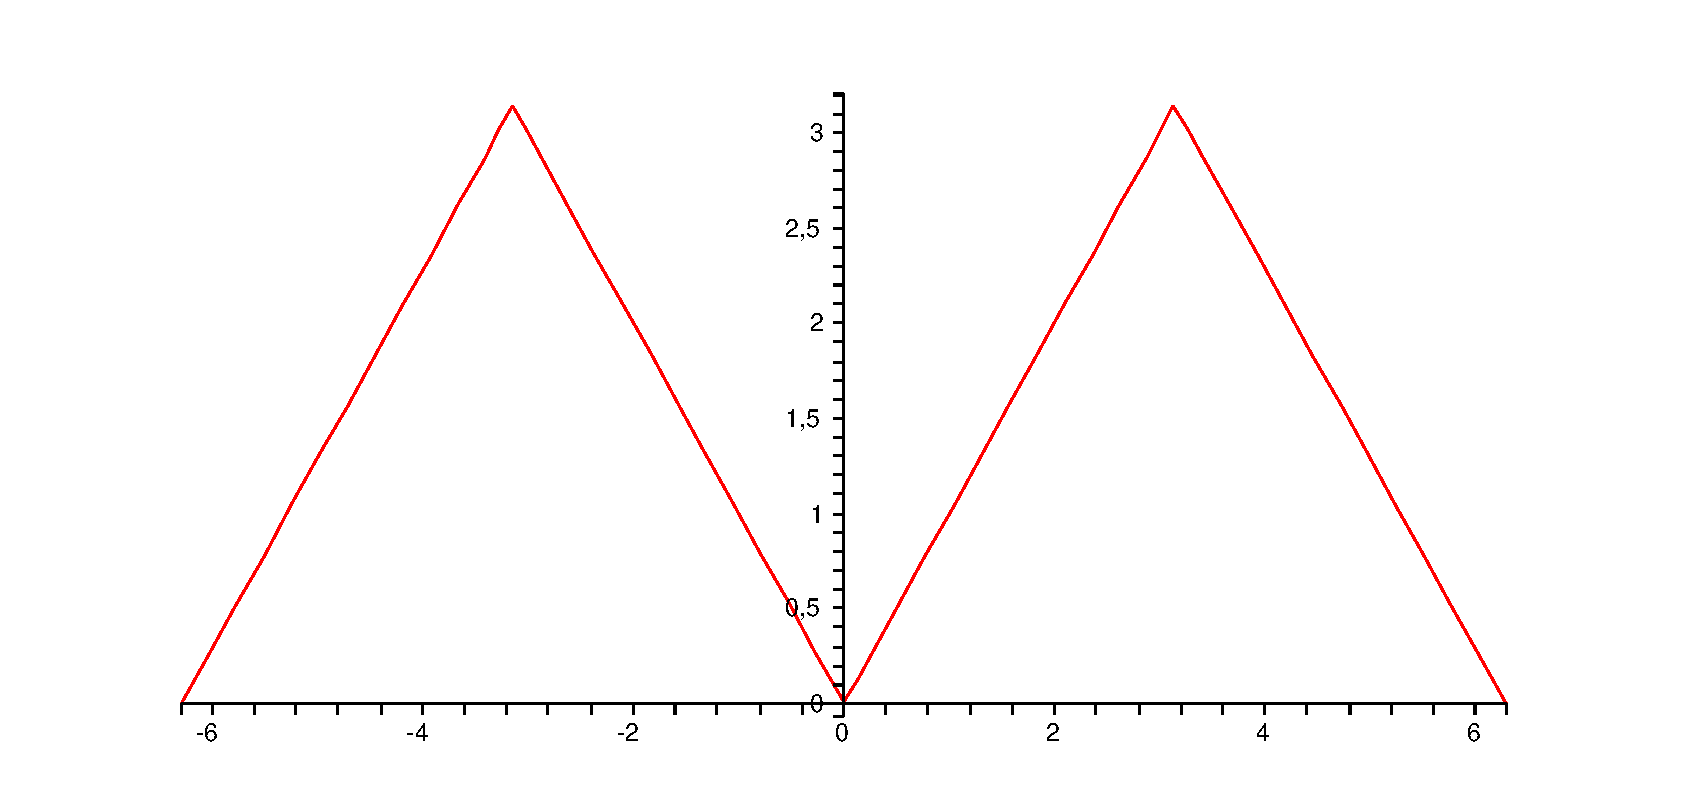
\epsfig{file=Figures/saegezahn.eps,scale=0.5}
   \caption{Die S\"agezahn-Funktion.}
  \label{fig:saegezahn.eps}
\end{figure}
\begin{enumerate}
\item Die Koeffizienten $a_n$ ergeben sich als 
      \\[0.3cm]
      \hspace*{0.5cm}
      $\displaystyle
        a_n  =  \bruch{1}{\pi} \cdot\int_0^{2\cdot\pi} s(x) \cdot \cos(n\!\cdot\!x)\,\dr x 
             =  \bruch{2}{\pi} \cdot\int_{0}^{\pi} s(x) \cdot \cos(n\!\cdot\!x)\,\dr x
             =  \bruch{2}{\pi} \cdot\int_{0}^{\pi} x \cdot \cos(n\!\cdot\!x)\,\dr x, 
      $
      \\[0.3cm]
      denn die Funktion $x \mapsto s(x) \cdot \cos(n\!\cdot\!x)\,\dr x$ ist einerseits
      periodisch mit der Periode $2\cdot\pi$ und andererseits gerade.
      Im Falle $n=0$ haben wir 
      \\[0.1cm]
      \hspace*{1.3cm}
        $\displaystyle a_0 = \bruch{2}{\pi} \cdot\int_{0}^{\pi} x \cdot \cos(0\!\cdot\!x)\,\dr x =
          \bruch{2}{\pi} \cdot\int_{0}^{\pi} x \,\dr x = 
          \bruch{2}{\pi} \cdot \bruch{x^2}{2} \,\bigg|_0^\pi = \bruch{2}{\pi} \cdot \bruch{\pi^2}{2} =\pi$.
      \\[0.1cm]
      Andernfalls berechnen wir das Integral  mit Hilfe partieller Integration.  Wir setzen
      $u'(x) = \cos(n\!\cdot\!x)$ und $v(x) = x$.  Dann gilt
      $u(x) = \frac{1}{n}\cdot \sin(n\!\cdot\!x)$ und $v'(x) = 1$, also haben wir f\"ur 
      $n \geq 1$
      \\[0.3cm]
      \hspace*{1.3cm}
      $
      \begin{array}[t]{lcl}
         a_n &= &\displaystyle \bruch{2}{\pi} \cdot\left( x \cdot \bruch{1}{n}\sin(n\!\cdot\!x) \bigg|_0^{\pi} - 
               \bruch{1}{n}\cdot \int_0^{\pi} \sin(n\!\cdot\!x)\,\dr x\right) \\[0.5cm]
             &= &\displaystyle \bruch{2}{\pi} \cdot\left(0 + \bruch{1}{n^2} \cdot \cos(n\!\cdot\!x)\, \bigg|_0^\pi\right) \\[0.5cm]
             &= &\displaystyle \bruch{2}{\pi} \cdot\bruch{1}{n^2}\cdot \Bigl( (-1)^n - 1 \Bigr), 
      \end{array}
      $
      \\[0.3cm]
      denn $\cos(n\cdot \pi) = (-1)^n$. Damit haben wir insgesamt
      \\[0.3cm]
      \hspace*{1.3cm}
      $a_0 = \pi$, \quad $a_{2\cdot n+1} = \bruch{-4}{\pi\cdot n^2}$ \quad und \quad $a_{2\cdot(n+1)} = 0$ \quad f\"ur $n\in \mathbb{N}$.
\item Die Koeffizienten $b_n$ ergeben sich als
      \\[0.3cm]
      \hspace*{1.3cm}
      $b_n  = \displaystyle \bruch{1}{\pi} \cdot\int_0^{2\cdot\pi} s(x) \cdot \sin(n\!\cdot\!x)\,\dr x = 0$
      \\[0.3cm]
      denn die Funktion $s(x) \cdot \sin(n\!\cdot\!x)$ ist sowohl periodisch mit der Periode $2\cdot\pi$ als auch ungerade.
\end{enumerate}
Insgesamt haben wir jetzt die Formel 
\\[0.3cm]
\hspace*{1.3cm}
$\displaystyle s(x) = \bruch{\pi}{2} - \bruch{4}{\pi} \cdot\sum\limits_{k=0}^\infty \bruch{1}{(2\!\cdot\!k+1)^2} \cdot \cos\bigl((2\!\cdot\!k+1)\cdot x\bigr)$
\\[0.3cm]
gefunden.  Setzen wir hier f\"ur $x$ den Wert $\pi$ ein, so ergibt sich wegen $\cos\bigl((2\!\cdot\!k+1)\cdot \pi\bigr) = - 1$
\\[0.1cm]
\hspace*{1.3cm}
$
\begin{array}[t]{clcl}
                & \pi & = & \bruch{\pi}{2} - \bruch{4}{\pi} \cdot\sum\limits_{k=0}^\infty \bruch{1}{(2\!\cdot\!k+1)^2} \cdot \cos\bigl((2\!\cdot\!k+1)\cdot \pi\bigr) \\[0.5cm]
\Leftrightarrow & \bruch{\pi}{2} & = &  \bruch{4}{\pi} \cdot\sum\limits_{k=0}^\infty \bruch{1}{(2\!\cdot\!k+1)^2} \\[0.5cm]
\Leftrightarrow & \bruch{\pi^2}{8} & = & \displaystyle \sum\limits_{k=0}^\infty \bruch{1}{(2\!\cdot\!k+1)^2}.
\end{array}
$
\\[0.3cm]
Damit sind wir jetzt in der Lage, die Reihe 
\\[0.2cm]
\hspace*{1.3cm}
$\ds \sigma := \sum\limits_{n=1}^\infty \frac{1}{n^2}$
\\[0.2cm]
zu berechnen.  Zun\"achst zerlegen wir die Reihe in einen Teil, der nur \"uber die geraden Indices 
l\"auft und einen Teil, der \"uber die ungeraden Indices l\"auft: 
\\[0.3cm]
\hspace*{1.3cm}
$
\begin{array}[t]{clcl}
                & \sigma & = & \displaystyle 
                  \sum\limits_{n=1}^\infty \bruch{1}{(2\!\cdot\!n)^2} \;+\; \sum\limits_{n=0}^\infty \bruch{1}{(2\!\cdot\!n+1)^2} \\[0.5cm]
\Leftrightarrow & \sigma & = & \displaystyle 
                  \bruch{1}{4}\cdot\sum\limits_{n=1}^\infty \bruch{1}{n^2} \;+\; \bruch{\pi^2}{8} \\[0.5cm]
\Leftrightarrow & \sigma & = & \displaystyle \bruch{1}{4} \cdot \sigma  \;+\; \bruch{\pi^2}{8} \\[0.3cm]
\Leftrightarrow & \bruch{3}{4}\cdot\sigma & = & \bruch{\pi^2}{8} \\[0.3cm]
\Leftrightarrow & \sigma & = & \bruch{\pi^2}{6} 
\end{array}
$
\\[0.3cm]
Damit haben wir also die Formel 
\\[0.3cm]
\hspace*{1.3cm} \colorbox{red}{\colorbox{orange}{\framebox{ $\ds\sum\limits_{n=1}^\infty \frac{1}{n^2} = \frac{\pi^2}{6}$}}}
\\[0.3cm]
gezeigt.  Die Frage nach dem Wert dieser Reihe war 1644 als \emph{Basel'sches Problem} von
Pietro Mengoli gestellt worden. 
F\"uhrende Mathematiker des 17-ten Jahrhunderts hatten sich erfolglos mit dieser Frage
besch\"aftigt.
Im Jahre 1735 gelang es Leonard Euler (1707 - 1783), dieses Problem zu l\"osen.

\exercise
Die Funktion $p$ sei auf dem Intervall $[-\pi,\pi]$ definiert durch
\\[0.1cm]
\hspace*{1.3cm}
$p(x) = x^2$.
\\[0.1cm]
Die Funktion werde so auf $\mathbb{R}$ fortgesetzt, dass die resultierende Funktion die Periode
$2\!\cdot\!\pi$ hat.  
\begin{enumerate}[(a)]
\item Berechnen Sie die Fourier-Reihe von $p$.
\item Berechnen Sie mit Hilfe der Fourier-Reihe von $p$ einen Wert f\"ur die Reihe
      \\[0.3cm]
      \hspace*{1.3cm}
      $\displaystyle \sum\limits_{n=1}^\infty \frac{1}{n^2}$. \eox
\end{enumerate}



%%% Local Variables: 
%%% mode: latex
%%% TeX-master: "analysis"
%%% End: 
